% !TEX TS-program = pdflatex
% !TEX encoding = UTF-8 Unicode

% This is a simple template for a LaTeX document using the "article" class.
% See "book", "report", "letter" for other types of document.

\documentclass[11pt]{article} % use larger type; default would be 10pt

\usepackage[utf8]{inputenc} % set input encoding (not needed with XeLaTeX)

%%% Examples of Article customizations
% These packages are optional, depending whether you want the features they provide.
% See the LaTeX Companion or other references for full information.

%%% PAGE DIMENSIONS
\usepackage{geometry} % to change the page dimensions
\geometry{a4paper} % or letterpaper (US) or a5paper or....
% \geometry{margin=2in} % for example, change the margins to 2 inches all round
% \geometry{landscape} % set up the page for landscape
%   read geometry.pdf for detailed page layout information

\usepackage{graphicx} % support the \includegraphics command and options
\usepackage{alltt}
\usepackage{wrapfig}
% \usepackage[parfill]{parskip} % Activate to begin paragraphs with an empty line rather than an indent

%%% PACKAGES
\usepackage{booktabs} % for much better looking tables
\usepackage{array} % for better arrays (eg matrices) in maths
\usepackage{amssymb}
\usepackage{paralist} % very flexible & customisable lists (eg. enumerate/itemize, etc.)
\usepackage{verbatim} % adds environment for commenting out blocks of text & for better verbatim
\usepackage{subfig} % make it possible to include more than one captioned figure/table in a single float
% These packages are all incorporated in the memoir class to one degree or another...

%%% HEADERS & FOOTERS
\usepackage{fancyhdr} % This should be set AFTER setting up the page geometry
\pagestyle{fancy} % options: empty , plain , fancy
\renewcommand{\headrulewidth}{0pt} % customise the layout...
\lhead{}\chead{}\rhead{}
\lfoot{}\cfoot{\thepage}\rfoot{}

%%% SECTION TITLE APPEARANCE
\usepackage{sectsty}
\allsectionsfont{\sffamily\mdseries\upshape} % (See the fntguide.pdf for font help)
% (This matches ConTeXt defaults)

%%% ToC (table of contents) APPEARANCE
\usepackage[nottoc,notlof,notlot]{tocbibind} % Put the bibliography in the ToC
\usepackage[titles,subfigure]{tocloft} % Alter the style of the Table of Contents
\renewcommand{\cftsecfont}{\rmfamily\mdseries\upshape}
\renewcommand{\cftsecpagefont}{\rmfamily\mdseries\upshape} % No bold!

%%% END Article customizations

%%% The "real" document content comes below...

\title{Numerical Analysis Project 1}
\author{Margaret Dorsey}
%\date{} % Activate to display a given date or no date (if empty),
         % otherwise the current date is printed 

\newenvironment{claim}[1]{\par\noindent\underline{Claim:}\space#1}{}
\newenvironment{proof}[1]{\par\noindent\underline{Proof:}\space#1}{\hfill $\blacksquare$}

\begin{document}
\maketitle

\section*{Positive Solutions of X}

\begin{claim}
There is exactly one positive solution for $x$.
\end{claim}
\begin{proof}

%% show f(0) < 0
We first note $f(0) < 0$ for all values of $k$ ,$\eta$, $\xi$ - when $x = 0$, the rest of the function $f(x)$ disappears, leaving us with $f(0) = -\xi$, a negative value, because $\xi$ represents ligand concentration, a physical quantity, and thus must be positive (because $0$ is a trivial case and negative values are non-physical).
%% find and demonstrate an x such that f(x) > 0, x is large
\par Additionally, for $x = \xi$, $f(x) > 0$, because $f(x) = \xi - \xi + \sum_{j=1}^{M} \frac{k_j \eta_j}{1+k_j\eta}$ in this case, where all of the sum terms are non-negative, and at least one is non-zero (otherwise it is modelling a trivial case where there is no amount of any binding molecules).
%% thus there is a root due to intermediate value theorem, f is continuous
\par Thus, by the intermediate value theorem, we know that $f$ has at least one positive root between $0$ and $\xi$. Calculating the derivative with respect to $x$ of $f$, we get
	$$f'(x) = 1 + \sum_{j=1}^{M} = \frac{k_j \eta_j}{(1+k_jx)^2}$$
%% show function is strictly increasing for positive x using the derivative
which by reasoning analogous to the above argument, is always positive for positive $x$. Thus $f(x)$ is strictly increasing for positive $x$, and due to Rolle's theorem, we know that $f(x)$ restricted to positive $x$ has at most one root, which completes the proof.
%%a strictly increasing function has at most one root, due to Rolle's Theorem
%% done

\end{proof}

\section*{Fixed Point Iteration}

\subsection*{Finding $g(x)$}

\subsubsection*{Case Testing}
%%show it works for case 1, not for case 2
%% discuss the problem here
%% use contraction theorem

\subsubsection*{Choosing $\alpha$}

%% find an alpha that works 

\begin{claim}
If $\alpha  = \sum_{j=1}^M k_jn_j$, the FPI always converges.
\end{claim}
\begin{proof}
\end{proof}


\section*{Newton's Method}

\subsection*{Test One Output}
%initial guess 1.6, what do you dislike about results
\begin{alltt}
Enter the intial guess: 1.6

--------------------------
 Newton
 -----------------------


i: 0	x: -1.124105012	value: 88.452818065
i: 1	x: -1.260131012	value: 46.182036757
i: 2	x: -1.570535828	value: 24.956847208
i: 3	x: -2.357298970	value: 14.010274589
i: 4	x: -4.536830098	value: 7.290560454
i: 5	x: -8.588461093	value: 1.729329152
i: 6	x: -10.061914568	value: 0.041604994
i: 7	x: -10.099003088	value: 0.000018410
i: 8	x: -10.099019514	value: 0.000000000

\end{alltt}

\subsection*{Test Two Output}
\subsubsection*{Output}
%initial guess 1.4999, discuss results
\begin{alltt}
Enter the intial guess: 1.4999

--------------------------
 Newton
 -----------------------


i: 0	x: -0.999876924	value: -81242.749956933
i: 1	x: -0.999753861	value: -40619.374953876
i: 2	x: -0.999507770	value: -20307.687427792
i: 3	x: -0.999015733	value: -10151.843615770
i: 4	x: -0.998032241	value: -5073.921612311
i: 5	x: -0.996067582	value: -2534.960417718
i: 6	x: -0.992147546	value: -1265.479442812
i: 7	x: -0.984344518	value: -630.738232506
i: 8	x: -0.968885874	value: -313.366310246
i: 9	x: -0.938552168	value: -154.678222468
i: 10	x: -0.880170250	value: -75.331900493
i: 11	x: -0.772155001	value: -35.661641481
i: 12	x: -0.587979613	value: -15.858623262
i: 13	x: -0.323256320	value: -6.099899665
i: 14	x: -0.056125978	value: -1.650760190
i: 15	x: 0.078909646	value: -0.189707093
i: 16	x: 0.098689910	value: -0.003059278
i: 17	x: 0.099019425	value: -0.000000818
i: 18	x: 0.099019514	value: -0.000000000

\end{alltt}


\subsection*{Test Three Output}
% guess 1.5, discuss results, they should be horrible
\begin{alltt}

Enter the intial guess: 1.5

--------------------------
 Newton
 -----------------------


i: 0	x: -1.000000000	value: -inf
i: 1	x: -nan	value: -nan

\end{alltt}


\subsection*{Test Four Output}
% guess 1.0, should be nice
\begin{alltt}

\end{alltt}

\subsection*{Analysis}
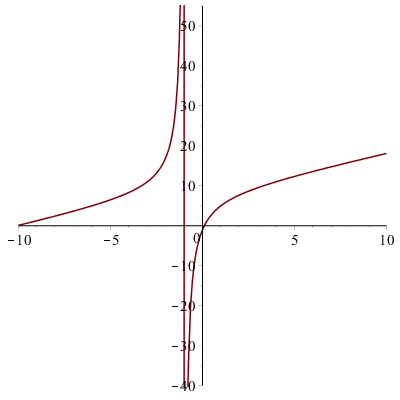
\includegraphics[scale=.5]{plots/newtongraph1.png}


\par For an initial guess of 1.6, the method successfully converged, however unfortunately it was to the negative root. For 1.499, the method converged (somewhat slowly, for newton's method) to the correct root, however 1.5 leads to division by zero. Examining the graph of f(x), the cause of this behavior becomes fairly apparent - as the positive side of the graph flattens and the slope of the tangent line approaches $0$, Newton's method tends to send $x_{n+1}$ through and across the singularity at $x = -1$, into the negative values of $x$. For $x$ before this jump across the singularity of $f(x)$, such as $1.4999$, the method, although displaced into negative $x$, can self-correct back towards the positive root. As the slope of $f(x)$ gets more and more positive approaching the positive root, Newton's method manages to converge more and more efficiently, as evidenced by the results of initial guess $1.0$.


\section*{Algorithm Comparison}

\subsection*{Output Evaluation}

\subsection*{Asymptotic Error Constant Calculation}

\subsection*{Test Case Results}

\subsection*{Conclusions and Preferred Algorithm}
 

\end{document}
